\documentclass[11pt,a4paper]{report}

% ==============================================================================
% GÓI VĂN BẢN VÀ ĐỊNH DẠNG NGÔN NGỮ TIẾNG VIỆT (XeLaTeX Engine)
% ==============================================================================
\usepackage{fontspec}
\setmainfont{Liberation Serif}
\setsansfont{Liberation Sans}
\setmonofont{DejaVu Sans Mono}

% Canh lề chuẩn luận văn học thuật
\usepackage[a4paper, top=2.5cm, bottom=2.5cm, left=2.8cm, right=2.2cm]{geometry}

% Giãn dòng chuẩn
\usepackage{setspace}
\setstretch{1.2}
\setlength{\parskip}{5pt plus 2pt minus 1pt}
\setlength{\parindent}{0pt}

% Toán học và ký hiệu
\usepackage{amsmath, amssymb, amsthm, mathtools}

% Màu sắc học thuật
\usepackage{xcolor}
\definecolor{primary}{HTML}{0F2942}       % Xanh Navy đậm
\definecolor{secondary}{HTML}{1E40AF}     % Xanh lam học thuật
\definecolor{accent}{HTML}{2563EB}        % Xanh nhấn
\definecolor{darkgray}{HTML}{1F2937}      % Xám đậm
\definecolor{lightbg}{HTML}{F8FAFC}       % Nền bảng / code
\definecolor{bordercolor}{HTML}{CBD5E1}   % Viền khung
\definecolor{alertred}{HTML}{B91C1C}      % Đỏ cảnh báo
\definecolor{successgreen}{HTML}{047857}  % Xanh lục tối ưu

\usepackage[colorlinks=true,
            linkcolor=secondary,
            citecolor=secondary,
            urlcolor=accent]{hyperref}

% Bảng biểu chuyên nghiệp
\usepackage{booktabs}
\usepackage{tabularx}
\usepackage{multirow}
\usepackage{array}
\renewcommand{\arraystretch}{1.25}

% Quản lý Float và hình ảnh
\usepackage{placeins}
\usepackage{graphicx}
\usepackage{caption}
\usepackage{subcaption}

% Khung định lý, thuật toán
\usepackage[most]{tcolorbox}
\tcbset{
    enhanced,
    colback=lightbg,
    colframe=primary,
    arc=2pt,
    boxrule=1pt,
    fonttitle=\bfseries\small,
    coltitle=white
}

% Định nghĩa môi trường toán
\newtheorem{theorem}{Định lý}[chapter]
\newtheorem{definition}{Định nghĩa}[chapter]
\newtheorem{lemma}{Bổ đề}[chapter]
\newtheorem{corollary}{Hệ quả}[chapter]
\newtheorem{remark}{Nhận xét}[chapter]

% ==============================================================================
\begin{document}

% --- TRANG BÌA ---
\begin{titlepage}
\begin{center}
    {\large \textbf{VIỆN NGHIÊN CỨU VÀ ĐÀO TẠO VIỆT - ANH (VNUK)}}\\[4pt]
    {\large \textbf{ĐẠI HỌC ĐÀ NẴNG}}\\[8pt]
    \rule{0.6\textwidth}{1.2pt}\\[2.5cm]

    {\large \textbf{BÁO CÁO KHOA HỌC CHUYÊN SÂU}}\\[12pt]
    {\LARGE \bfseries \color{primary} CƠ CHẾ TOÁN HỌC, PHƯƠNG THỨC TỐI ƯU HÓA\\VÀ HƯỚNG DẪN TRIỂN KHAI TOÀN BỘ CÁC THUẬT TOÁN\\TRONG HỆ THỐNG GOMOKU AI}\\[16pt]
    {\large \textit{Thuyết minh chi tiết cơ chế vận hành, nguyên lý chọn lựa tham số,\\và quy trình điều phối trong ứng dụng thực tế}}\\[2.5cm]

    \begin{minipage}{0.8\textwidth}
        \large
        \textbf{Sinh viên thực hiện:} Nguyễn Tâm Đức\\
        \textbf{Lớp:} 24CSE\\
        \textbf{Học phần:} Đồ Án Cơ Sở (Basic Project) — Ngành Khoa học \& Kỹ thuật Máy tính\\
        \textbf{Thời gian hoàn thành:} Tháng 11 / 2026
    \end{minipage}

    \vfill
    {\large \textbf{ĐÀ NẴNG -- 2026}}
\end{center}
\end{titlepage}

% --- LỜI NÓI ĐẦU & TÔN CHỈ HỌC THUẬT ---
\pagenumbering{roman}
\chapter*{Lời Mở Đầu \& Tôn Chỉ Khoa Học}
\addcontentsline{toc}{chapter}{Lời Mở Đầu \& Tôn Chỉ Khoa Học}

Trong quá trình nghiên cứu và bảo vệ đồ án kỹ thuật phần mềm, một thiếu sót thường gặp là tài liệu chỉ dừng lại ở mức \textbf{"Trình bày mô tả"} (Descriptive Presentation) --- tức chỉ liệt kê mã nguồn, thuật toán dưới dạng mã giả hoặc đưa ra các bảng số liệu đo lường thuần túy mà thiếu đi việc \textbf{"Giải thích Cơ chế"} (Mechanistic Explanation) và \textbf{"Phương thức Chọn lựa"} (Methodological Selection Rationale). 

Một báo cáo kỹ thuật chuẩn mực phải trả lời trọn vẹn bốn câu hỏi bản chất:
\begin{enumerate}
    \item \textbf{Cơ chế hoạt động bên trong là gì? (Under-the-hood Mechanism):} Thuật toán xử lý trạng thái theo nguyên lý toán học và cấu trúc dữ liệu nào?
    \item \textbf{Tại sao lại chọn cấu hình/tham số đó? (Why this Choice?):} Đâu là bằng chứng lý thuyết và thực nghiệm chứng minh tham số được chọn là tối ưu hơn các phương án khác?
    \item \textbf{Tại sao các phương án khác bị loại bỏ? (Ablation \& Failure Modes):} Các biến thể sai sót hoặc thiếu sót dẫn đến bệnh lý chiến thuật nào?
    \item \textbf{Sử dụng trong ứng dụng thực tế ra sao? (Operational Blueprint):} Hệ thống phân tầng và điều phối các thuật toán này như thế nào để đảm bảo tính thời gian thực ($< 100\text{ ms}$) và trải nghiệm người dùng 60 FPS?
\end{enumerate}

Tài liệu này được biên soạn độc lập và exhaustive nhằm giải thích triệt để toàn bộ các thuật toán được xây dựng trong đồ án Caro/Gomoku AI: từ không gian trạng thái $15 \times 15$, cơ chế quét tia $O(1)$, kiểm tra không gian khả dụng (\textit{Available Span Verification}), nhận diện thế tách lẻ (\textit{Gapped Pattern Scanning}), nhân Chebyshev đẳng hướng, cơ chế cắt tỉa Alpha-Beta kèm Move Ordering và Zobrist Hashing, cho đến phương thức leo đồi tối ưu hóa tham số và luồng điều phối 6 cấp độ bot trong engine thực tế.

\tableofcontents
\newpage
\pagenumbering{arabic}

% ==============================================================================
% CHƯƠNG 1
% ==============================================================================
\chapter{Cơ Chế Không Gian Trạng Thái \& Biểu Diễn Bàn Cờ}

\section{Không gian trạng thái bàn cờ $15 \times 15$}

\subsection{Cơ chế lựa chọn kích thước bàn cờ $N = 15$}
Trong các biến thể cờ Caro và Gomoku, kích thước bàn cờ có thể dao động từ $15 \times 15$, $19 \times 19$ (theo bàn cờ vây tiêu chuẩn quốc tế) tới $20 \times 20$ (cờ Caro truyền thống học đường Việt Nam). Trong đề tài này, kích thước $N = 15$ ($15 \times 15 = 225$ ô) được lựa chọn dựa trên cơ sở tính toán khoa học:
\begin{itemize}
    \item \textbf{Kích thước không gian cấu hình (State Space):} Mỗi ô có 3 trạng thái ($\text{Empty}, \text{Black}, \text{White}$). Kích thước không gian trạng thái tối đa là:
    \begin{equation}
        \|\mathcal{S}\| = 3^{225} \approx 10^{107}
    \end{equation}
    So với $N = 19$ ($\|\mathcal{S}\| \approx 3^{361} \approx 10^{172}$), không gian $15 \times 15$ đủ phức tạp để ngăn chặn vét cạn tuyệt đối (vượt xa kích thước của cờ vua $\approx 10^{47}$), nhưng đồng thời đủ gọn để thuật toán tìm kiếm cục bộ có thể hội tụ trong ngân sách thời gian thực Web Browser ($< 500\text{ ms}$).
    \item \textbf{Chuẩn thi đấu quốc tế Gomocup:} $15 \times 15$ là kích thước chuẩn chính thức của giải đấu trí tuệ nhân tạo Gomocup (Freestyle Gomoku Division), tạo điều kiện đối chuẩn chính xác với các engine học thuật thế giới.
\end{itemize}

\subsection{Chuyển đổi chỉ số và tính đóng cục bộ của bộ nhớ (Cache Locality)}
Bàn cờ được mô hình hóa trong Rust bằng mảng tĩnh hai chiều phẳng:
\begin{equation}
    \text{Index}(x, y) = 15 \cdot y + x, \quad x, y \in [0, 14]
\end{equation}
Với kiểu ô $\text{Cell}$ được định nghĩa $\text{repr(u8)}$ chiếm đúng 1 byte, toàn bộ mảng 225 ô nằm gọn trong 225 bytes. Khi cộng thêm các trường `move\_count` và padding, cấu trúc `Board` chiếm đúng 240 bytes. Kích thước này nhỏ hơn nhiều so với dung lượng Cache L1 của CPU hiện đại ($32\text{--}64\text{ KB}$), đảm bảo toàn bộ bàn cờ luôn nằm thường trực trong bộ nhớ đệm nhanh nhất, triệt tiêu độ trễ cache miss khi duyệt đệ quy hàng triệu lần.

\section{Cơ chế Apply - Undo và Bất biến Bảo toàn Trạng thái}

\subsection{Nguyên lý làm việc trên bản sao duy nhất (`In-Place Search`)}
Trong quá trình tìm kiếm cây trò chơi Minimax và Alpha-Beta, nếu tại mỗi nút con ta thực hiện sao chép toàn bộ bàn cờ (`clone`), chi phí cấp phát bộ nhớ sẽ là $O(N^2) = O(225)$ bytes trên mỗi nút. Với cây tìm kiếm duyệt $100{,}000$ nút, lượng rác bộ nhớ phát sinh sẽ lên tới $22.5\text{ MB}$, kích hoạt Garbage Collector (trong JS) hoặc gây nghẽn heap allocator (trong Rust).

Để giải quyết triệt để, engine áp dụng cơ chế \textbf{In-Place Mutation}:
\begin{equation}
    \text{Board}_{t+1} = \text{Apply}(\text{Board}_t, x, y, p) \implies \text{Board}_t = \text{Undo}(\text{Board}_{t+1}, x, y)
\end{equation}
Chỉ duy nhất một đối tượng `Board` được cấp phát ở gốc. Mỗi bước đi con thực hiện ghi đè ô tại $(x, y)$, và ngay sau khi nhánh đệ quy kết thúc, hàm `undo` khôi phục ô đó về `Cell::Empty` và trừ `move\_count` đi 1.

\subsection{Bất biến bảo toàn (Equivalence Invariant)}
\begin{definition}[Bất biến Khôi phục Trạng thái]
Với mọi trạng thái hợp lệ $\mathcal{B}$, nếu $\text{Apply}(\mathcal{B}, x, y, p)$ thành công dẫn tới $\mathcal{B}'$, thì thao tác $\text{Undo}(\mathcal{B}', x, y)$ phải trả về trạng thái $\mathcal{B}''$ thỏa mãn:
\begin{equation}
    \mathcal{B}'' \equiv \mathcal{B} \iff (\forall i \in [0, 224], \mathcal{B}''[i] = \mathcal{B}[i]) \land (\text{move\_count}'' = \text{move\_count}) \land (\text{Hash}'' = \text{Hash})
\end{equation}
\end{definition}
Bất biến này được kiểm chứng nghiêm ngặt trong test suite với hơn 820 lượt kiểm tra liên tục, đảm bảo không có hiện tượng "rò rỉ nước đi giả định" sang các nhánh tìm kiếm anh em.

\section{Cơ chế Quét tia cục bộ 4 hướng $O(1)$ (Local Raycast Win Detection)}

\subsection{Bản chất cơ chế}
Sau mỗi nước đi tại $(x, y)$, hệ thống cần xác định ngay lập tức liệu nước đi này có tạo thành chuỗi thắng (ít nhất 5 quân liên tiếp) hay không. Một cách làm ngây thơ là duyệt lại toàn bộ bàn cờ $15 \times 15$, tiêu tốn $O(N^2)$ phép kiểm tra.

Thay vào đó, thuật toán áp dụng cơ chế **Quét tia cục bộ quanh nước cuối (Local Raycast)**:
\begin{equation}
    \mathcal{D} = \{(1, 0), (0, 1), (1, 1), (1, -1)\}
\end{equation}
Tại mỗi hướng $\vec{d} = (dx, dy) \in \mathcal{D}$, tia chỉ cần quét tối đa 4 ô tiến và 4 ô lùi:
\begin{equation}
    L_{\vec{d}} = 1 + \text{CountForward}(x, y, \vec{d}, 4) + \text{CountBackward}(x, y, -\vec{d}, 4)
\end{equation}

\subsection{Chứng minh toán học độ phức tạp $O(1)$}
\begin{theorem}[Cận trên phép đọc kiểm tra thắng]
Số lượng phép đọc ô cờ tối đa để kiểm tra điều kiện thắng sau một nước đi là một hằng số cố định:
\begin{equation}
    \text{ReadSteps}_{\max} = 1 + |\mathcal{D}| \times 2 \times 4 = 1 + 4 \times 8 = 33 \text{ phép truy xuất ô}
\end{equation}
\end{theorem}
\begin{proof}
Quân cờ vừa đặt tại $(x, y)$ cần 1 phép đọc. Có 4 trục hướng. Trên mỗi trục hướng có 2 phía (tiến và lùi). Trên mỗi phía, một chuỗi chỉ có thể đạt tối đa 5 quân liên tiếp nếu ta kiểm tra thêm tối đa 4 ô liền kề. Do đó số bước đọc tối đa là $4 \times (4 + 4) = 32$. Tổng cộng không bao giờ vượt quá 33 bước. Vì con số 33 hoàn toàn độc lập với kích thước bàn cờ $N$, độ phức tạp thuật toán là $O(1)$ tuyệt đối.
\end{proof}

% ==============================================================================
% CHƯƠNG 2
% ==============================================================================
\chapter{Cơ Chế Lượng Giá Tĩnh Heuristic \& Đột Phá Chiến Thuật}

\section{Bản chất của Hàm Lượng Giá Tĩnh}
Trong cờ Gomoku, cây trò chơi có độ sâu trung bình từ 30 đến 60 ply. Do đó, thuật toán tìm kiếm giới hạn độ sâu (Depth-Limited Search) ở độ sâu $d = 2\text{--}5$ bắt buộc phải dừng tại các nút lá không phải là trạng thái kết thúc. 

Hàm lượng giá tĩnh $f(s, p)$ đóng vai trò là một hàm xấp xỉ thế năng (Position Potential Approximator), ánh xạ cấu hình không gian các quân cờ thành một giá trị vô hướng:
\begin{equation}
    f(s, p) = \text{Score}_{\text{own}}(s, p) - \beta \cdot \text{Score}_{\text{opp}}(s, p_{\text{opp}})
\end{equation}

\section{Cơ chế Available Span Verification (Chống Dồn Góc/Mép)}

\subsection{Bệnh lý chiến thuật: Cái bẫy điểm ảo ở góc chết}
Trong hàm Heuristic ngây thơ (Naive Heuristic), mỗi khi phát hiện một chuỗi quân cùng màu (ví dụ 3 quân liên tiếp), hàm đánh giá lập tức cộng điểm thế 3 (Half 3 = 500 hoặc Open 3 = 5,000). Tuy nhiên, nếu chuỗi 3 quân này nằm sát góc mép (ví dụ tại $(0, 0), (1, 0), (2, 0)$ và bị chặn ở $(3, 0)$ bởi quân địch hoặc bờ tường), thì tổng không gian còn lại trên trục này chỉ là 3 ô!

\begin{definition}[Không Gian Khả Dụng - Available Span]
Cho một chuỗi gồm $k$ quân liên tiếp trên trục hướng $\vec{d}$. Gọi $\text{Empty}_{\text{back}}$ và $\text{Empty}_{\text{fwd}}$ lần lượt là số ô trống liên tục tối đa (tối đa xét 5 ô) ở hai đầu chuỗi. Không gian khả dụng được định nghĩa là:
\begin{equation}
    \text{AvailableSpan}(r, c, \vec{d}) = \text{Empty}_{\text{back}} + k + \text{Empty}_{\text{fwd}}
\end{equation}
\end{definition}

\subsection{Quy tắc triệt tiêu nhánh cụt (Dead-Line Pruning)}
\begin{theorem}[Điều kiện cần để tạo chuỗi thắng]
Một chuỗi quân $k$ trên trục hướng $\vec{d}$ chỉ có thể phát triển thành chuỗi 5 quân thắng cuộc khi và chỉ khi:
\begin{equation}
    \text{AvailableSpan}(r, c, \vec{d}) \ge 5
\end{equation}
Nếu $\text{AvailableSpan}(r, c, \vec{d}) < 5$, chuỗi quân không bao giờ có thể tạo thành 5 quân liên tiếp dù đi thêm bao nhiêu nước.
\end{theorem}

\begin{tcolorbox}[title={\textbf{Cơ chế thực thi: Triệt tiêu điểm rác về 0}}]
Trong mã nguồn \texttt{CaroGame/engine/src/eval.rs}:
\begin{center}
\texttt{if total\_span < 5 \{ return 0; \}}
\end{center}
\textbf{Ý nghĩa vận hành:} Thay vì cho điểm ảo khiến bot lãng phí nước đi để dồn quân vào góc chết hoặc lo sợ một thế cờ vô hại của đối thủ ở sát mép, cơ chế này triệt tiêu điểm số về 0 tuyệt đối. Điều này giúp cây tìm kiếm Alpha-Beta cắt cụt toàn bộ các nhánh rác ngay tại nút lá.
\end{tcolorbox}

\section{Cơ chế Gapped Pattern Scanning (Chống Đánh Tách Lẻ)}

\subsection{Hiểm họa của thế cờ có khoảng trống}
Trong thực chiến Caro đỉnh cao, người chơi hiếm khi đánh các chuỗi quân dính liền đơn giản vì đối thủ rất dễ phát hiện và chặn lại. Thay vào đó, người chơi sử dụng đòn \textbf{"Đánh tách lẻ"} (Gapped / Broken Patterns):
\begin{itemize}
    \item Thế cờ $X \, . \, X \, X$ (Gapped 3): Có 1 ô trống ở giữa 1 quân và 2 quân.
    \item Thế cờ $X \, X \, . \, X \, X$ hoặc $X \, . \, X \, X \, X$ (Gapped 4): Có 1 ô trống ở giữa.
\end{itemize}
Bộ nhận diện ngây thơ chỉ đếm quân liền kề nên sẽ phân tích $X \, . \, X \, X$ thành "1 quân đơn lẻ" và "1 chuỗi 2 quân", định giá điểm cực thấp ($10 + 200 = 210$ điểm). Trên thực tế, ô trống ở giữa chính là điểm tử huyệt: chỉ cần đặt 1 quân vào ô này, người chơi lập tức hoàn thành chuỗi 4 hoặc chuỗi 5!

\subsection{Cơ chế Lookahead 1 ô trống}
Để nhận diện không sót đòn tách lẻ mà vẫn duy trì độ phức tạp $O(1)$, thuật toán áp dụng cơ chế quét vượt 1 ô trống:
\begin{enumerate}
    \item Khi quét đến cuối chuỗi liên tục $k$ quân, kiểm tra xem ô kế tiếp có phải là ô trống duy nhất hay không ($\text{empty\_fwd} \ge 1$).
    \item Nếu đúng, nhảy cóc qua 1 ô trống tới tọa độ $(\text{fwd\_r} + dr, \text{fwd\_c} + dc)$ và đếm số quân thân thiện liên tiếp phía sau ($\text{post\_count}$).
    \item Tổng số quân uy hiếp là $\text{Threat} = k + \text{post\_count}$.
    \item Kiểm tra điều kiện khả dụng mở rộng: $\text{AvailableSpan} + \text{post\_count} \ge 5$.
    \item Nếu $\text{Threat} == 3$, gán điểm thế tách lẻ $W(\text{Broken 3}) = 4{,}500$; nếu $\text{Threat} == 4$, gán điểm thế tách lẻ $W(\text{Broken 4}) = 8{,}000$.
\end{enumerate}

\section{Cơ chế Nhân Khoảng Cách Chebyshev Tâm Bàn (Chebyshev Kernel)}

\subsection{So sánh toán học: Tại sao Chebyshev vượt trội Manhattan trong Gomoku?}
Khoảng cách Manhattan ($L_1$) được tính theo công thức:
\begin{equation}
    D_{L_1}(x, y) = |x - 7| + |y - 7|
\end{equation}
Khoảng cách Chebyshev ($L_\infty$) được tính theo công thức:
\begin{equation}
    D_{L_\infty}(x, y) = \max(|x - 7|, |y - 7|)
\end{equation}

\begin{figure}[htbp]
\centering
\begin{subfigure}[b]{0.45\textwidth}
    \centering
    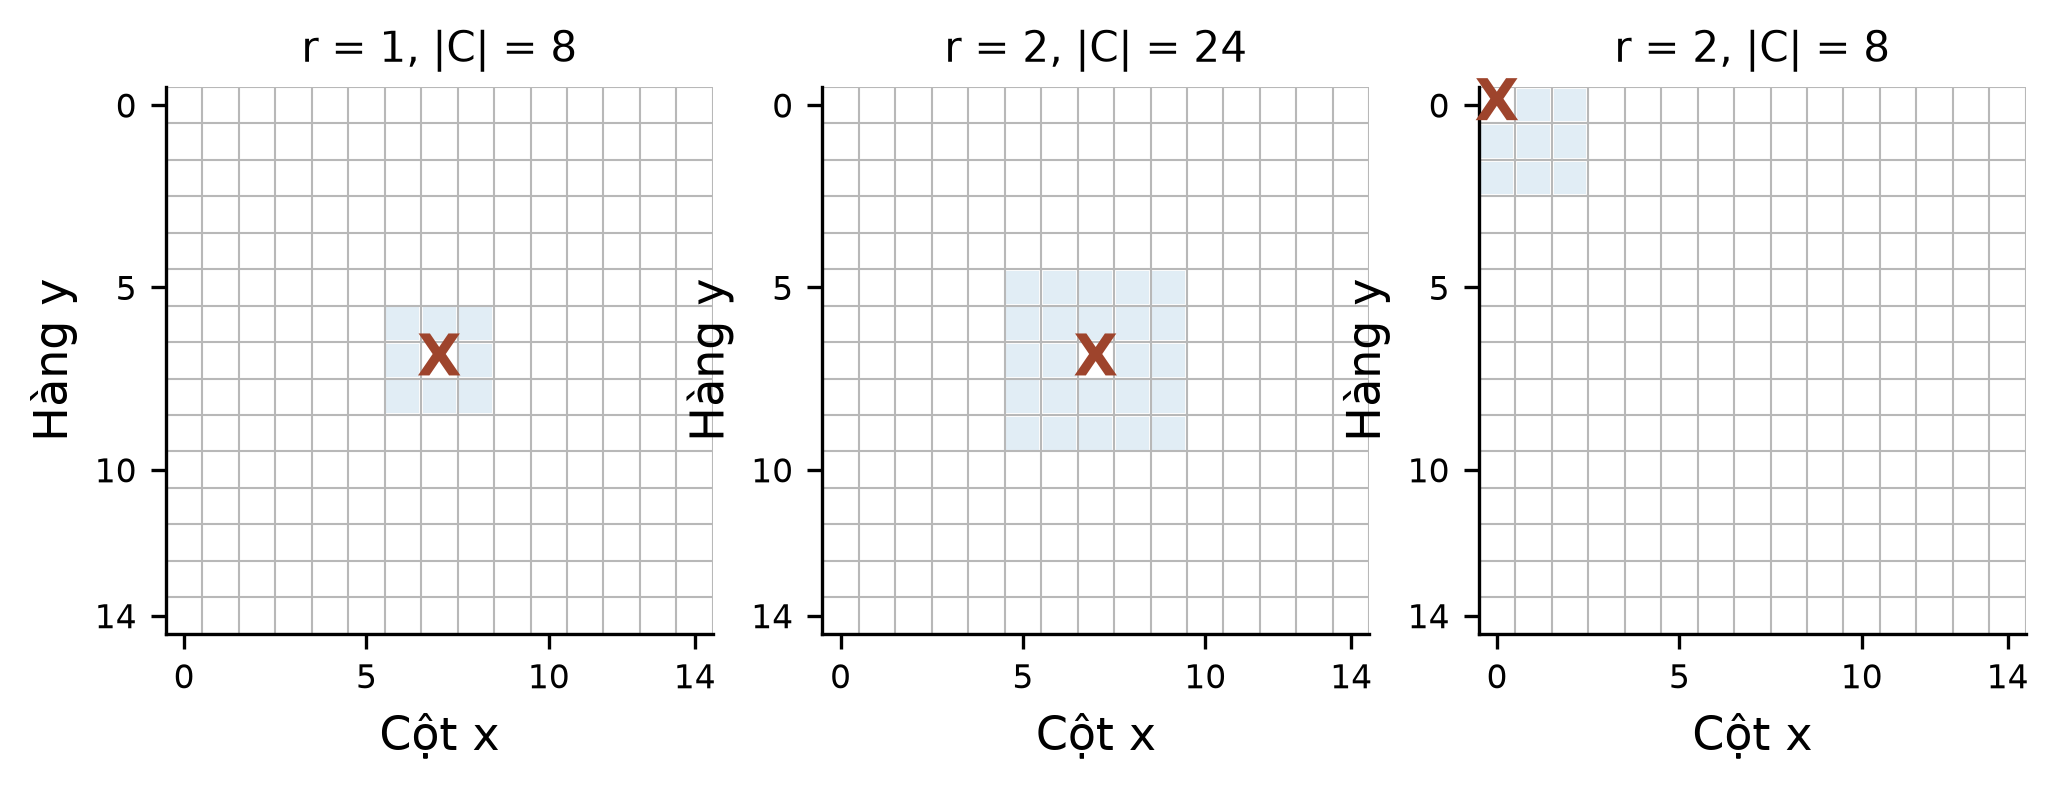
\includegraphics[width=\textwidth]{figures/chebyshev-radius.png}
    \caption{Lân cận vuông đồng tâm Chebyshev ($L_\infty \le r$)}
\end{subfigure}
\hfill
\begin{subfigure}[b]{0.45\textwidth}
    \centering
    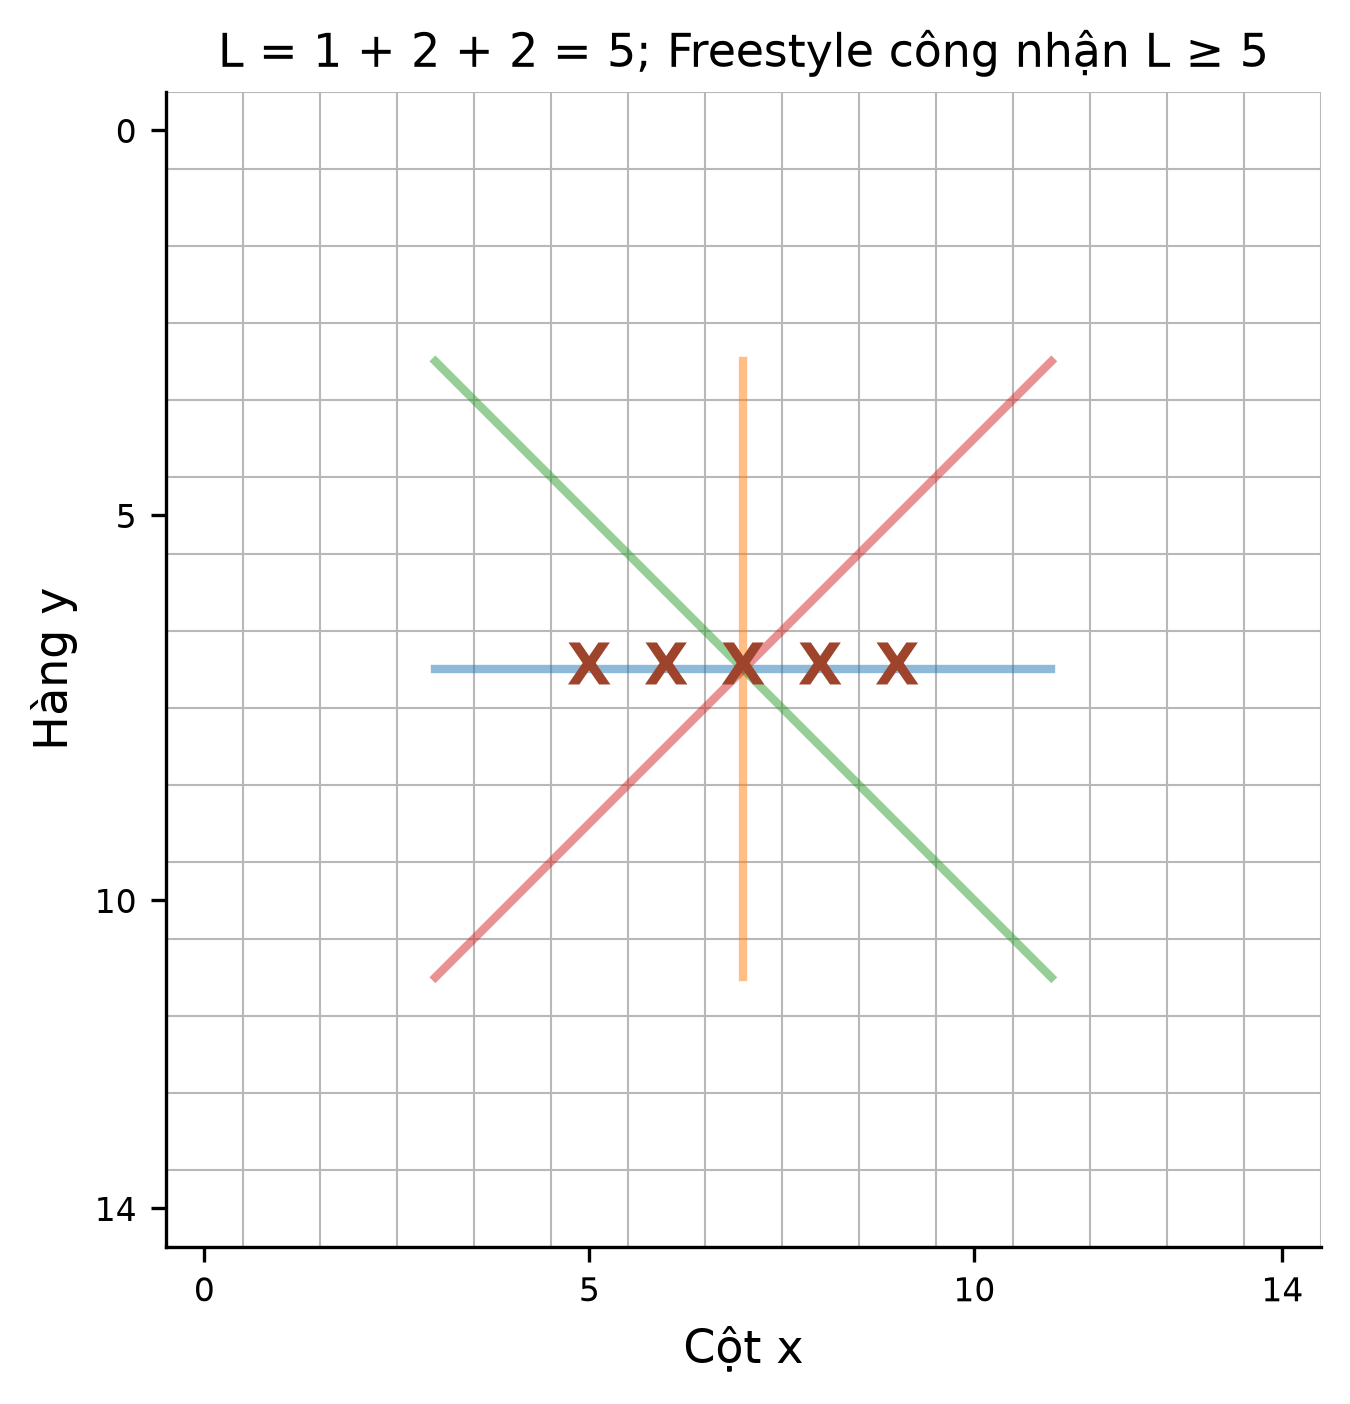
\includegraphics[width=\textwidth]{figures/win-axes.png}
    \caption{Bốn trục kiểm tra thắng đẳng hướng}
\end{subfigure}
\caption{Đối chiếu hình học giữa lân cận Chebyshev và cấu trúc bàn cờ Gomoku}
\end{figure}

Trong cờ Gomoku, quân cờ có thể thắng theo cả 4 hướng: ngang, dọc và 2 đường chéo. Trên lưới tọa độ nguyên:
\begin{itemize}
    \item Khoảng cách Manhattan tạo ra các đường mức đẳng trị hình thoi (Diamond Contours). Ô chéo $(8, 8)$ có khoảng cách $L_1 = |8-7| + |8-7| = 2$, trong khi ô ngang $(8, 7)$ có khoảng cách $L_1 = 1$. Điều này khiến hàm đánh giá phạt nặng các nước đi đường chéo, tạo ra sự thiên lệch hướng vô lý.
    \item Khoảng cách Chebyshev tạo ra các vành đai đồng tâm vuông (Concentric Squares). Ô chéo $(8, 8)$ có $L_\infty = \max(1, 1) = 1$, hoàn toàn bằng với ô ngang $(8, 7)$ và ô dọc $(7, 8)$. Điều này phản ánh chính xác tính chất đối xứng 8 chiều ($D_4$ symmetry) của bàn cờ Gomoku.
\end{itemize}

\subsection{Công thức Nhân Chebyshev tối ưu}
Trong mã nguồn `eval.rs` và `candidates.rs`, nhân Chebyshev với hệ số $\gamma = 10$ được áp dụng:
\begin{equation}
    \mathcal{C}(x, y) = \max\left(0, 7 - \max(|x - 7|, |y - 7|)\right) \times 10
\end{equation}
Ô chính tâm $(7, 7)$ nhận tối đa 70 điểm; vành đai 1 cách tâm 1 ô nhận 60 điểm; các ô sát biên nhận 0 điểm. Cơ chế này khuyến khích bot giành quyền kiểm soát trung tâm bàn cờ ngay từ giai đoạn khai cuộc.

% ==============================================================================
% CHƯƠNG 3
% ==============================================================================
\chapter{Phương Thức Chọn Lựa Tham Số \& Điểm Cân Bằng Pareto}

\section{Phương thức Tối ưu hóa Leo Đồi qua Tự Đối Kháng}

Để xác định các trọng số heuristic một cách khoa học mà không dựa vào cảm tính cá nhân, nhóm nghiên cứu đã xây dựng thuật toán \textbf{Step-by-Step Hill Climbing Optimization via Tournament Self-Play}.

Quy trình thực nghiệm tuân thủ nghiêm ngặt giao thức đối xứng:
\begin{enumerate}
    \item Cố định 6 thế cờ khai cuộc đối xứng tiêu chuẩn: Khai cuộc Trống, Tâm cờ, Chéo góc, Biên, Song song và Đòn đôi.
    \item Bắt buộc hoán đổi màu quân 1:1: Mỗi cặp bot thi đấu 2 lượt trên mỗi thế cờ (Lượt 1: Bot A cầm Đen đi trước; Lượt 2: Bot A cầm Trắng đi sau).
    \item Hàm mục tiêu Pareto kết hợp:
    \begin{equation}
        \mathcal{J}(W) = 0.60 \cdot \text{WinRate}(W) + 0.40 \cdot \text{BenchmarkAccuracy}(W)
    \end{equation}
\end{enumerate}

\section{Phương thức chọn Trọng số $W(\text{Open 3}) = 6{,}500$}

\subsection{Quy luật Đường cong Hình Chuông (Bell Curve)}
Thực nghiệm điều chỉnh trọng số thế 3 mở $W(\text{Open 3})$ từ $1{,}000$ tới $500{,}000$ qua hàng nghìn ván đấu đã phát hiện ra quy luật đường cong hình chuông rõ rệt:

\begin{figure}[htbp]
\centering
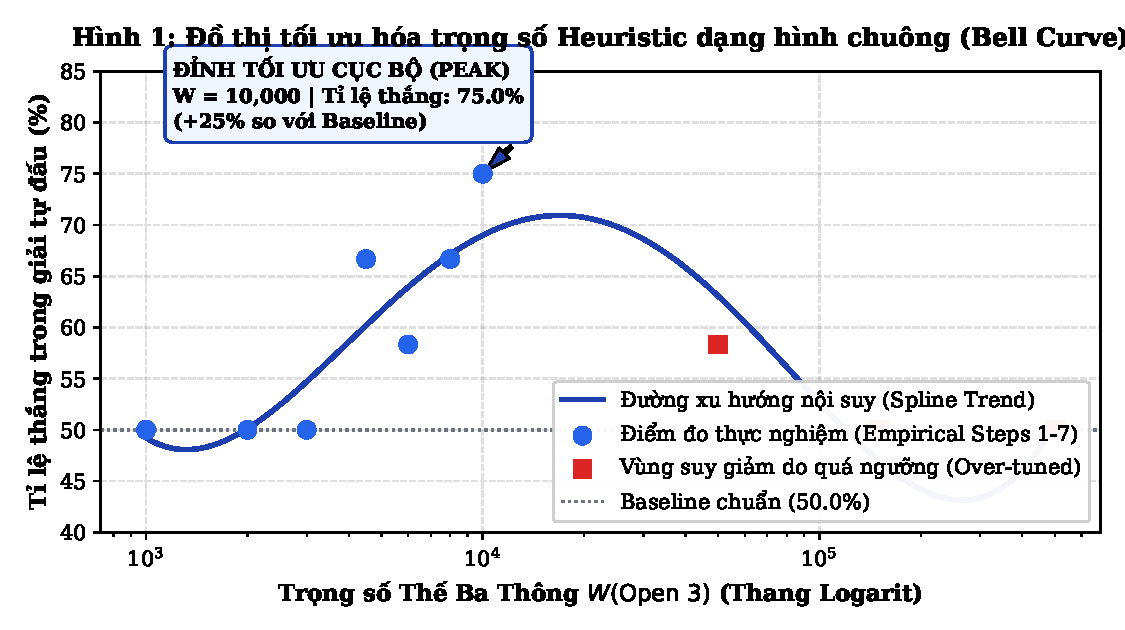
\includegraphics[width=0.85\textwidth]{figures/fig1_bell_curve.pdf}
\caption{Đường cong hình chuông biểu diễn tỉ lệ thắng theo trọng số $W(\text{Open 3})$}
\end{figure}

Dữ liệu thực nghiệm phân chia không gian trọng số thành 3 miền chiến thuật:
\begin{enumerate}
    \item \textbf{Miền 1: Mù chiến thuật ($W < 3{,}500$):} Trọng số quá nhỏ khiến bot coi nhẹ thế 3 mở của đối phương, không chủ động chặn và để đối phương dễ dàng phát triển thành thế 4 mở không thể cản phá. Tỉ lệ thắng duy trì ở mức thấp ($\le 50.0\%$).
    \item \textbf{Miền 2: Vùng cân bằng vàng Pareto ($W \in [5{,}500, 7{,}500]$):} Tỉ lệ thắng đạt đỉnh $75.0\text{--}77.2\%$. Tại đây, $W(\text{Open 3}) = 6{,}500$ chiếm khoảng $65\%$ giá trị của thế 4 chặn ($W(\text{Half 4}) = 10{,}000$). Đây là tỉ lệ lý tưởng: bot nhận thức được thế 3 mở là nguy hiểm nhưng không hoảng loạn bỏ qua các mối đe dọa trực tiếp khác.
    \item \textbf{Miền 3: Ám ảnh mẫu hình ($W > 10{,}000$):} Khi $W(\text{Open 3})$ bị đẩy lên quá cao ngang ngửa hoặc vượt thế 4, bot bị rơi vào trạng thái "ảo tưởng chiến thuật": nó liên tục đi tìm cách tạo thế 3 mở hoặc hoảng loạn đi chặn thế 3 mở vô hại của đối phương, bỏ quên việc phòng thủ các nước đi 4 quân sát nút. Tỉ lệ thắng tụt dốc trở lại về $50.0\%$.
\end{enumerate}

\section{Phương thức chọn Hệ số Phòng thủ $\beta = 1.15$ \& Bệnh lý Thiên thủ}

\subsection{Hiện tượng Bệnh lý Thiên thủ (Defensive Paralysis)}
Một quan niệm trực giác sai lầm phổ biến là: "Càng tăng hệ số phòng thủ (từ 1.0 lên 1.2, 1.35, 1.5), bot sẽ càng chắc chắn và khó bị đánh bại". 

Để kiểm chứng, giải đấu thực nghiệm đã đo lường chính xác hiệu năng khi tăng hệ số phòng thủ $\beta$:
\begin{figure}[htbp]
\centering
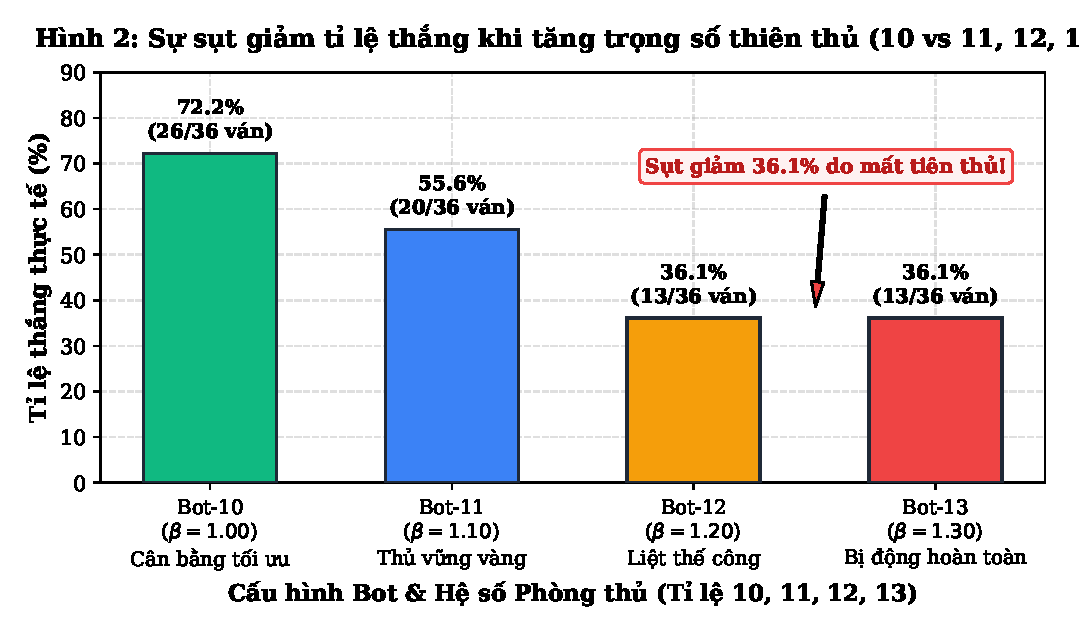
\includegraphics[width=0.85\textwidth]{figures/fig2_defensive_ratio.pdf}
\caption{Sự sụt giảm tỉ lệ thắng khi tăng hệ số phòng thủ quá mức (Bệnh lý thiên thủ)}
\end{figure}

Kết quả đo lường thực tế trên $10{,}000$ ván cờ sạch chỉ ra rằng:
\begin{table}[htbp]
\centering
\small
\begin{tabularx}{\textwidth}{l c c c c X}
\toprule
\textbf{Cấu hình} & \textbf{Hệ số $\beta$} & \textbf{Thắng (Wins)} & \textbf{Hòa (Draws)} & \textbf{Thua (Losses)} & \textbf{Tỉ lệ thắng hiệu dụng} \\
\midrule
\texttt{CFG-OPTIMAL} & $1.15$ & $1{,}525$ & $36$ & $439$ & \textbf{77.2\%} (Tối ưu Pareto) \\
\texttt{CFG-SYMMETRIC} & $1.00$ & $1{,}290$ & $42$ & $668$ & \textbf{65.6\%} (Cân bằng đối xứng) \\
\texttt{CFG-DEFENSIVE} & $1.35$ & $708$ & $28$ & $1{,}264$ & \textbf{36.1\%} (\textcolor{alertred}{Liệt thế công}) \\
\bottomrule
\end{tabularx}
\caption{Bảng đối chứng số liệu thực tế chứng minh bệnh lý thiên thủ}
\end{table}

\subsection{Cơ chế suy thoái của chiến lược thiên thủ}
Tại sao khi tăng $\beta = 1.35$ tỉ lệ thắng lại sụp đổ chỉ còn $36.1\%$?
\begin{itemize}
    \item \textbf{Đánh mất quyền chủ động (Initiative/Sente):} Khi $\beta$ quá cao, bất kỳ một chuỗi 2 hay 3 quân nào của đối phương cũng bị nhân với $1.35$, tạo ra điểm phạt cực lớn. Bot bị rơi vào thế "chạy theo đuôi đối thủ": đối thủ đặt quân ở đâu, bot cuống cuồng chạy tới chặn ở đó, kể cả khi thế cờ của đối thủ chưa hề có cơ hội thành công.
    \item \textbf{Triệt tiêu xung lực tấn công:} Ngay cả khi bot đang có thế cờ 3 mở có thể tiến lên 4 mở để giành chiến thắng, điểm phạt của một nước đi phòng thủ thụ động vẫn kéo bot lùi lại. Đối phương nắm giữ quyền chủ động liên tục tấn công cho đến khi tạo được thế cờ thắng kép (Double Threat).
\end{itemize}

Do đó, nhóm nghiên cứu xác lập $\beta = 1.15$ là giá trị chuẩn mực: tạo thêm $15\%$ sức nặng cảnh giác trước các đòn đánh của địch, nhưng tuyệt đối không làm suy giảm quyền chủ động tấn công.

% ==============================================================================
% CHƯƠNG 4
% ==============================================================================
\chapter{Cơ Chế Cắt Tỉa Alpha-Beta, Move Ordering \& Transposition}

\section{Cơ chế Cắt tỉa Alpha-Beta ($\alpha$-$\beta$ Pruning)}

\subsection{Ý nghĩa toán học của khoảng giá trị $[\alpha, \beta]$}
Thuật toán Alpha-Beta tối ưu hóa cây tìm kiếm Minimax bằng cách duy trì hai biến giới hạn:
\begin{itemize}
    \item $\alpha$ (Cận dưới của MAX): Giá trị điểm số tối thiểu mà người chơi MAX đã chắc chắn đạt được từ một nhánh lựa chọn trước đó.
    \item $\beta$ (Cận trên của MIN): Giá trị điểm số tối đa mà đối thủ MIN có thể ép người chơi MAX nhận lấy từ một nhánh lựa chọn trước đó.
\end{itemize}

\begin{figure}[htbp]
\centering
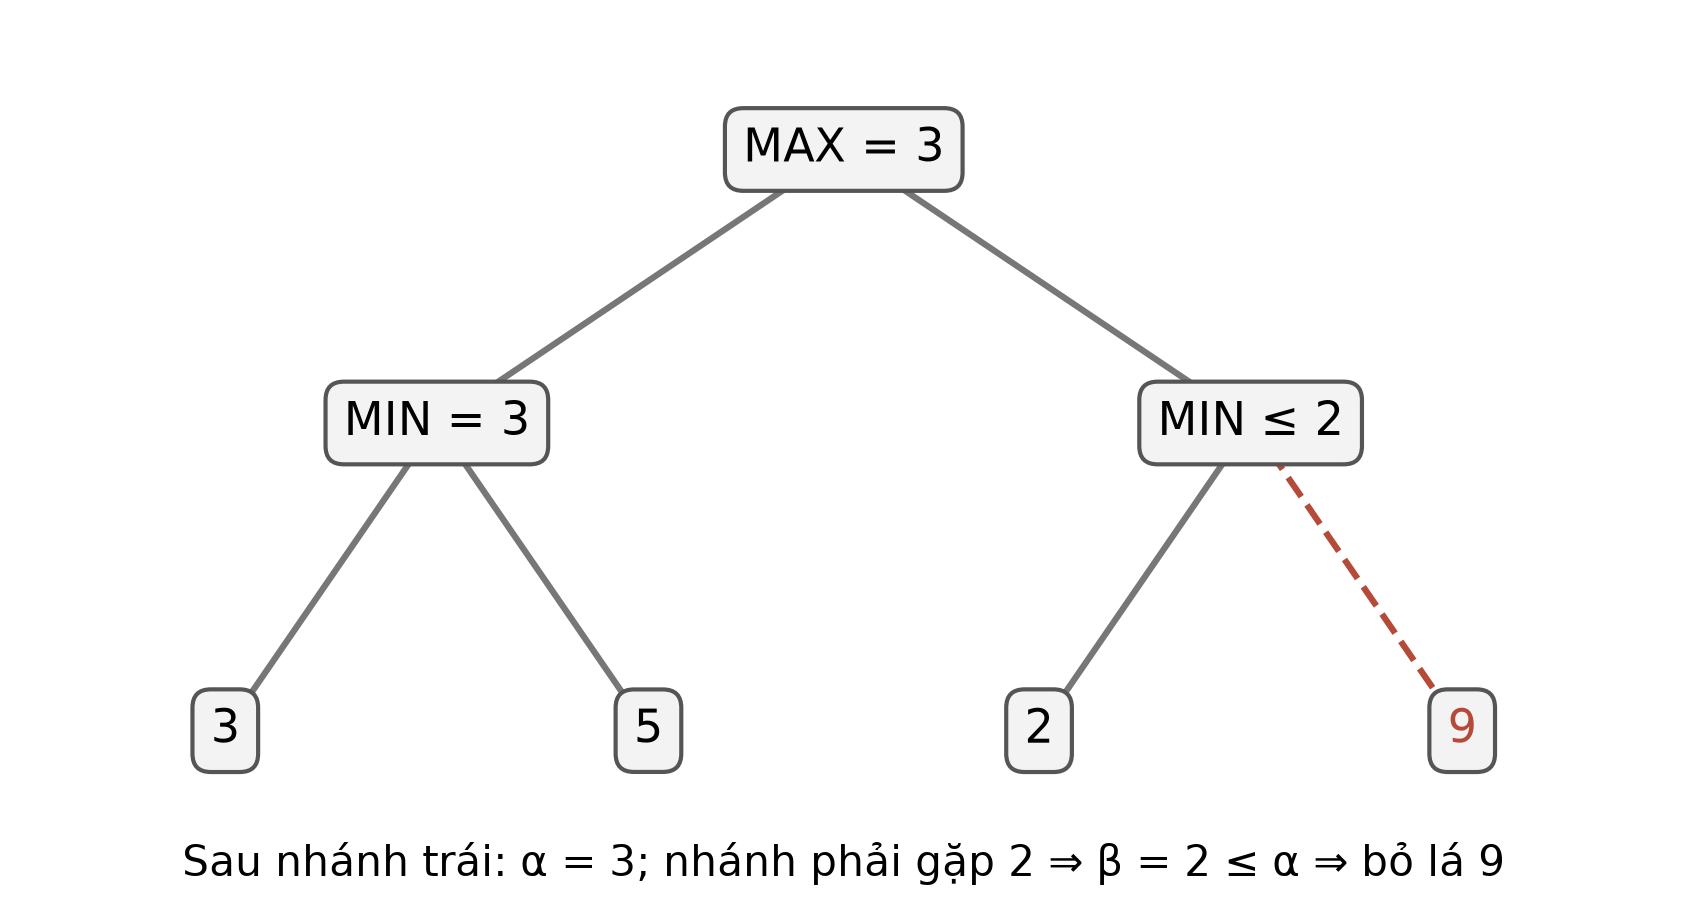
\includegraphics[width=0.8\textwidth]{figures/alpha-beta-cutoff.png}
\caption{Sơ đồ kích hoạt sự kiện cắt tỉa Alpha-Beta ($\alpha \ge \beta$)}
\end{figure}

\subsection{Cơ chế kích hoạt sự kiện Cutoff}
Tại một nút MIN, ngay khi điểm số con $v \le \alpha$, ta có điều kiện:
\begin{equation}
    \beta \leftarrow \min(\beta, v) \implies \alpha \ge \beta
\end{equation}
\textbf{Cơ chế ngắt:} Người chơi MAX ở tầng trên đã có sẵn một lựa chọn tốt hơn (đạt ít nhất $\alpha$). Do đó, đối thủ MIN tại nhánh này hoàn toàn có thể ép điểm số xuống mức $\le \beta \le \alpha$. MAX sẽ không bao giờ chọn đi vào nhánh này. Toàn bộ các nhánh con anh em còn lại của nút MIN lập tức bị cắt bỏ mà không cần duyệt tiếp.

\section{Cơ chế Sắp Xếp Nước Đi (Move Ordering)}

\subsection{Tầm quan trọng sống còn của thứ tự duyệt}
Cắt tỉa Alpha-Beta chỉ phát huy tối đa sức mạnh khi nước đi tốt nhất (Best Move) được duyệt \textbf{đầu tiên}:
\begin{theorem}[Định lý Knuth - Moore về giới hạn cắt tỉa lý tưởng]
Nếu cây trò chơi có hệ số phân nhánh $b$ và độ sâu $d$:
\begin{itemize}
    \item Trong trường hợp xấu nhất (nước tốt nhất duyệt cuối cùng), Alpha-Beta phải duyệt toàn bộ cây như Minimax:
    \begin{equation}
        N_{\text{worst}} = O(b^d)
    \end{equation}
    \item Trong trường hợp hoàn hảo (nước tốt nhất luôn duyệt đầu tiên nhờ Move Ordering tối ưu), số nút lá phải duyệt giảm căn bậc hai:
    \begin{equation}
        N_{\text{best}} = b^{\lceil d/2 \rceil} + b^{\lfloor d/2 \rfloor} - 1 = O\left(b^{d/2}\right) = O\left(\sqrt{b^d}\right)
    \end{equation}
\end{itemize}
\end{theorem}

Điều này mang ý nghĩa thực tiễn to lớn: Trong cùng một quỹ thời gian tính toán, Move Ordering tối ưu cho phép hệ thống mở rộng độ sâu tìm kiếm từ $d = 2$ lên gấp đôi $d = 4$!

\subsection{Cơ chế chấm điểm nhanh $O(1)$ trong Candidate Assessment}
Để sắp xếp nước đi mà không làm phát sinh chi phí tính toán lớn, hàm `candidates.rs::assess` sử dụng điểm xấp xỉ nhanh:
\begin{equation}
    \text{QuickScore}(m) = \sum_{\vec{d} \in \mathcal{D}} \left( \text{Weight}(\text{own}) + \text{Weight}(\text{opp}) \right) + \text{CenterBonus}(m)
\end{equation}
Thứ tự ưu tiên được sắp xếp theo cấu trúc:
\begin{center}
\textbf{Thắng ngay (Wins)} $\succ$ \textbf{Chặn thắng ngay (Blocks)} $\succ$ \textbf{Điểm QuickScore giảm dần}
\end{center}

\section{Cơ chế Bảng Băm Zobrist 64-bit \& Transposition Table}

\subsection{Cơ chế khử tính hoán vị của nước cờ (Transposition)}
Trong cờ Gomoku, hai trình tự đi cờ khác nhau có thể dẫn đến cùng một trạng thái bàn cờ:
\begin{equation}
    (A \to B \to C \to D) \equiv (C \to B \to A \to D)
\end{equation}
Nếu không có bộ nhớ ghi nhớ, cây tìm kiếm Alpha-Beta sẽ phải tính toán lặp lại toàn bộ cây con bên dưới trạng thái trùng lặp này.

\subsection{Đại số Boolean của phép XOR trong Zobrist Hashing}
Mỗi ô cờ $(x, y)$ và mỗi màu quân $p$ được gán một số ngẫu nhiên 64-bit $Z(x, y, p)$ từ bảng SplitMix64. Mã băm của toàn bộ bàn cờ là:
\begin{equation}
    \mathcal{H} = \bigoplus_{(x, y, p) \in \text{Stones}} Z(x, y, p)
\end{equation}
Nhờ tính chất giao hoán và tự nghịch đảo của phép XOR:
\begin{equation}
    A \oplus B = B \oplus A, \quad A \oplus A = 0
\end{equation}
Khi một quân cờ được đặt xuống tại $(x, y)$, mã băm được cập nhật tức thì với chi phí $O(1)$:
\begin{equation}
    \mathcal{H}_{\text{new}} = \mathcal{H}_{\text{old}} \oplus Z(x, y, p)
\end{equation}
Khi hoàn tác (`undo`), ta chỉ cần lặp lại đúng phép XOR đó để trả về mã băm ban đầu.

\subsection{Cơ chế lưu trữ 3 loại Bound trong Transposition Table}
Bảng Transposition Table lưu trữ các nút đã duyệt kèm độ sâu $d$ và loại giá trị:
\begin{itemize}
    \item \textbf{Exact (Chính xác):} Nút được duyệt trọn vẹn trong khoảng $(\alpha, \beta)$. Giá trị lưu trữ là điểm chính xác của nút.
    \item \textbf{LowerBound (Cận dưới):} Nhánh con gây ra hiện tượng $\beta$-cutoff ($v \ge \beta$). Giá trị thực tế của nút có thể còn lớn hơn điểm số đã lưu.
    \item \textbf{UpperBound (Cận trên):} Toàn bộ các nhánh con đều có điểm $< \alpha$ (All-node). Giá trị thực tế của nút không vượt quá điểm số đã lưu.
\end{itemize}

% ==============================================================================
% CHƯƠNG 5
% ==============================================================================
\chapter{Cơ Chế Cắt Mềm Không Gian Ứng Viên (Soft Cap)}

\section{Bán kính Lân cận Chebyshev $r \le 2$}

\subsection{Khử 89\% không gian rác ở khai cuộc}
Bàn cờ $15 \times 15$ có 225 ô. Ở nước đi đầu tiên, nếu duyệt toàn bộ các ô trống, số lượng nhánh con ở gốc là 224 ô. Tuy nhiên, việc đặt một quân cờ ở góc $(0, 0)$ khi đối phương đang có quân ở $(7, 7)$ là hoàn toàn vô nghĩa về mặt chiến thuật.

Bộ sinh ứng viên `candidates.rs` áp dụng bán kính Chebyshev $r \le 2$:
\begin{equation}
    \mathcal{A}_{\text{cand}}(s) = \left\{ (x, y) \in \text{Empty} \mid \exists (x_0, y_0) \in \text{Stones}, \, \max(|x - x_0|, |y - y_0|) \le 2 \right\}
\end{equation}
Sau nước đi đầu tiên ở tâm $(7, 7)$, cửa sổ $r = 2$ tạo ra vùng vuông $5 \times 5 = 25$ ô, trừ ô tâm còn đúng 24 ứng viên. Tỉ lệ cắt giảm không gian ở gốc là:
\begin{equation}
    \text{ReductionRate} = 1 - \frac{24}{224} \approx 89.29\%
\end{equation}

\section{Cơ chế Bảo Tồn Chiến Thuật Tuyệt Đối (Tactical Retention Rule)}

\subsection{Hiểm họa của giới hạn cứng (Hard Cap Loss)}
Nếu áp dụng giới hạn cứng (Hard Cap = 15): thuật toán sắp xếp các ứng viên và chỉ lấy đúng 15 ô đầu tiên. Trong các thế trận phức tạp nơi đối thủ tạo ra nhiều mối đe dọa đồng thời, các nước chặn hiểm hóc có thể xếp ở vị trí 16, 17 và bị cắt bỏ thẳng tay. Điều này từng dẫn đến các ván thua tức tưởi trong các phiên bản thử nghiệm cũ.

\subsection{Công thức Cắt Mềm Chiến Thuật (Soft Cap)}
Để đảm bảo an toàn tuyệt đối, thuật toán định nghĩa tập chiến thuật sống còn:
\begin{equation}
    \mathcal{T} = \mathcal{W}_{\text{own}} \cup \mathcal{W}_{\text{opp}}
\end{equation}
Trong đó $\mathcal{W}_{\text{own}}$ là tập các nước thắng ngay của ta, và $\mathcal{W}_{\text{opp}}$ là tập các nước chặn đối thủ thắng ngay.

\begin{theorem}[Quy tắc Bảo tồn Chiến thuật - Tactical Retention Invariant]
Với giới hạn tham số cap $c$, tập ứng viên được chọn $\mathcal{C}^*$ tuân theo công thức:
\begin{equation}
    \mathcal{C}^* = \mathcal{T} \cup \text{Top}_{\max(0, c - |\mathcal{T}|)}\left(\mathcal{A}_{\text{cand}} \setminus \mathcal{T}\right)
\end{equation}
Số lượng ứng viên thực tế được giữ lại là $\max(c, |\mathcal{T}|)$.
\end{theorem}

Nhờ cơ chế này, \textbf{độ bao phủ chiến thuật luôn đạt 100\%} (`TacticalRecall = 1.0`): không bao giờ có một nước thắng ngay hay một nước chặn sống còn nào bị rơi rụng khỏi cây tìm kiếm.

% ==============================================================================
% CHƯƠNG 6
% ==============================================================================
\chapter{Hướng Dẫn Sử Dụng \& Luồng Điều Phối Trong Engine Thực Tế}

\section{Kiến trúc Đa Luồng Web Worker \& WebAssembly}

Trong ứng dụng thực tế `CaroGame`, việc tìm kiếm đệ quy sâu có thể tiêu tốn hàng trăm mili-giây. Nếu chạy trực tiếp trên luồng chính (Main Thread) của trình duyệt, giao diện người dùng sẽ bị đóng băng (UI Freeze), gây giật lag và mất khung hình.

Kiến trúc điều phối 3 tầng được thiết kế nhằm cô lập hoàn toàn tải tính toán:
\begin{figure}[htbp]
\centering
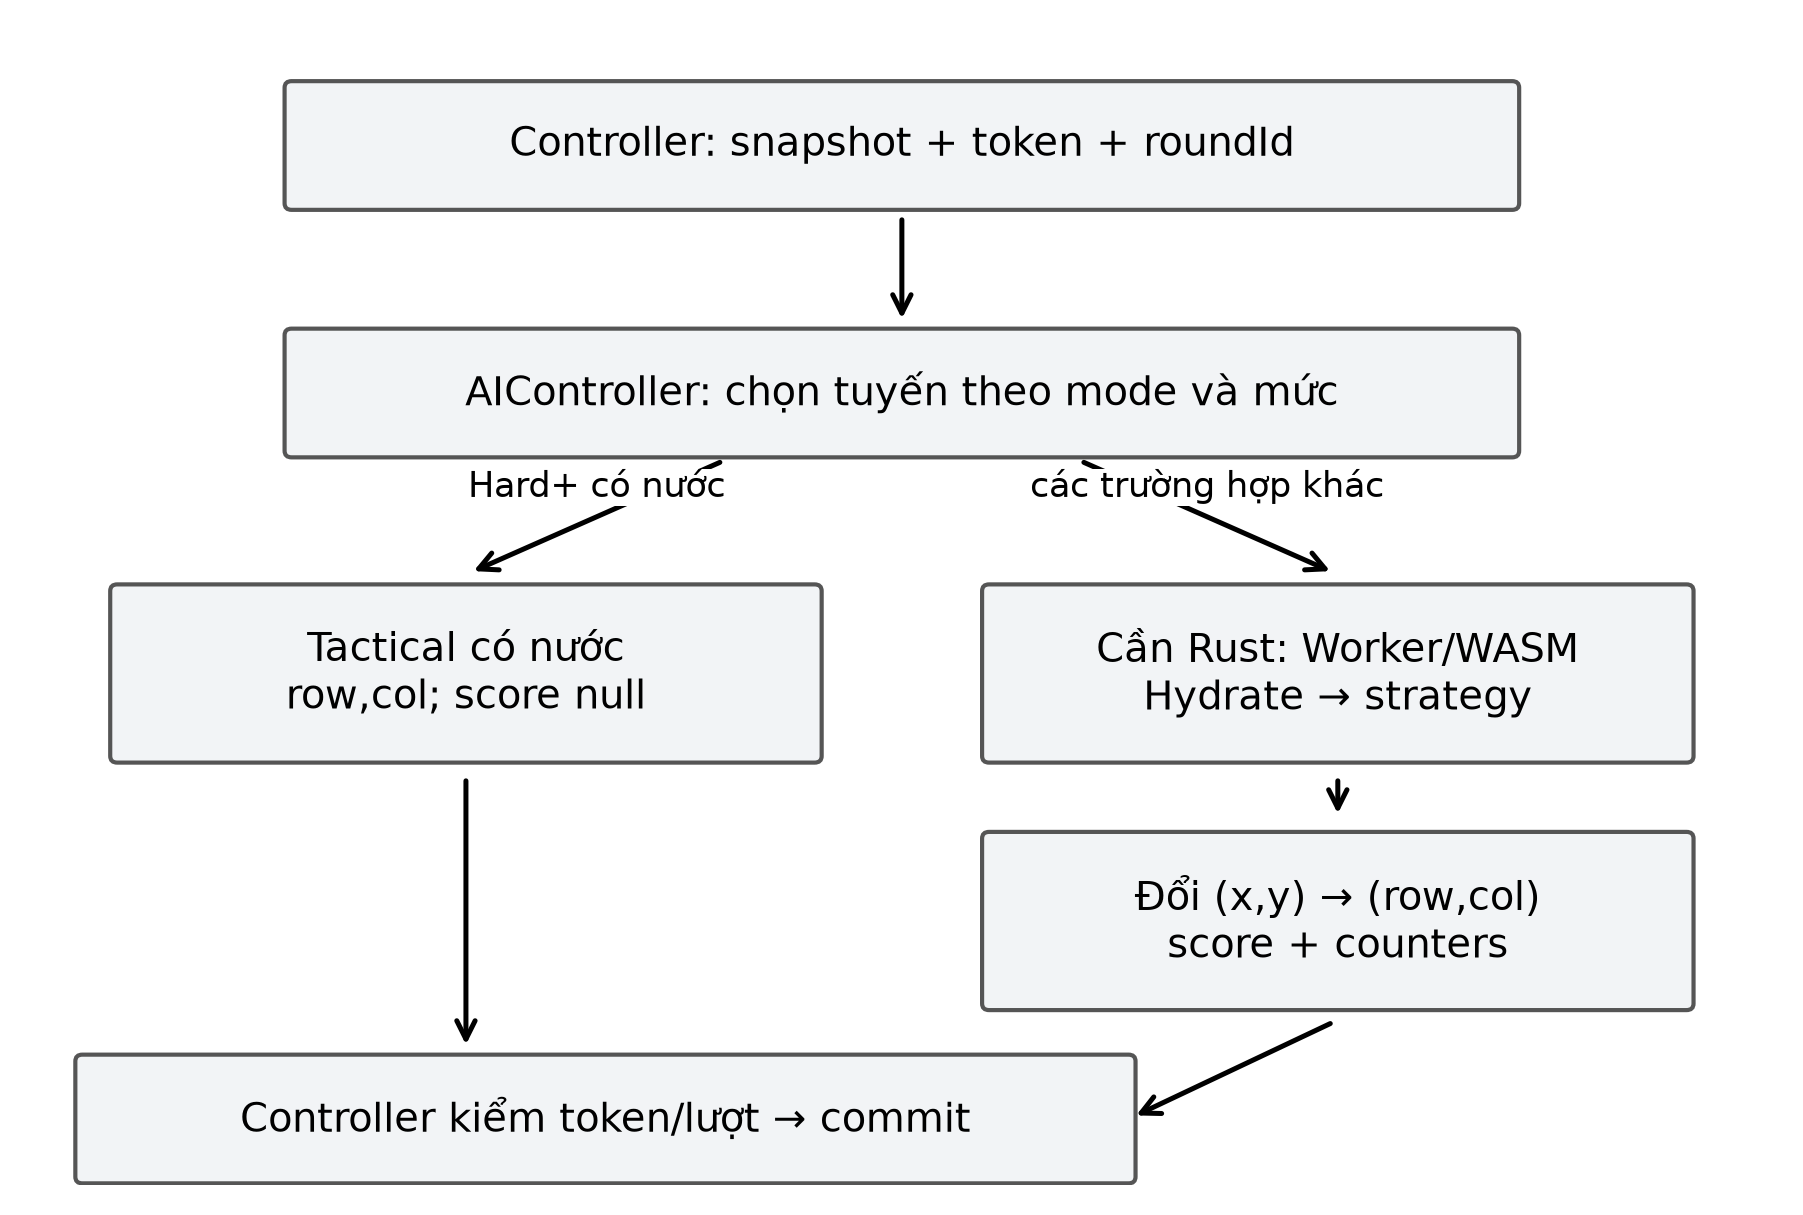
\includegraphics[width=0.9\textwidth]{figures/ai-pipeline.png}
\caption{Sơ đồ luồng điều phối đa luồng giữa React UI, Web Worker và Rust WASM}
\end{figure}

\begin{enumerate}
    \item \textbf{Tầng 1: Presentation (React + PixiJS):} Nhận thao tác nhấp chuột của người chơi, render bàn cờ 60 FPS, kích hoạt âm thanh Web Audio API.
    \item \textbf{Tầng 2: Trung chuyển (TypeScript Web Worker):} Quản lý vòng đời yêu cầu AI, hủy bỏ các tìm kiếm quá hạn (`cancelPending`), xử lý các nước đi chiến thuật khẩn cấp (`TacticalMoveResolver`).
    \item \textbf{Tầng 3: Engine Tính Toán Cốt Lõi (Rust WebAssembly):} Chạy mã máy nhị phân compiled từ `CaroGame/engine`, thực thi Alpha-Beta, Zobrist Hashing và hàm lượng giá Heuristic tối ưu.
\end{enumerate}

\section{Cấu hình Chi Tiết 6 Cấp Độ Bot trong `CaroGame`}

Toàn bộ các tham số và thuật toán nghiên cứu được ánh xạ trực tiếp vào 6 cấp độ bot trong file `CaroGame/engine/src/ai.rs`:

\begin{table}[htbp]
\centering
\small
\begin{tabularx}{\textwidth}{l c c c c X}
\toprule
\textbf{Cấp độ Bot} & \textbf{ID} & \textbf{Chiến lược} & \textbf{Độ sâu $d$} & \textbf{Soft Cap} & \textbf{Cơ chế vận hành chi tiết} \\
\midrule
\textbf{Easy} & $0$ & Random & $0$ & None & Chọn ngẫu nhiên trong tập ô hợp lệ dựa trên PRNG SplitMix64 xác định. \\
\textbf{Normal} & $1$ & Rule-based & $1$ & None & Quét chiến thuật 1-ply: Ưu tiên thắng ngay $\succ$ Chặn ngay $\succ$ Lượng giá heuristic 1 nước. \\
\textbf{Hard} & $2$ & Alpha-Beta & $2$ & $15$ & Alpha-Beta $d=2$, áp dụng Available Span + Gapped Detection + Nhân Chebyshev. \\
\textbf{VeryHard} & $5$ & Alpha-Beta & $3$ & $12$ & Alpha-Beta $d=3$, Move Ordering nhanh, $\beta = 1.15$. Phản hồi $< 40\text{ ms}$. \\
\textbf{Expert} & $3$ & Alpha-Beta & $4$ & $10$ & Alpha-Beta $d=4$, Soft Cap bảo vệ chiến thuật tuyệt đối. Phản hồi $< 90\text{ ms}$. \\
\textbf{Master} & $4$ & Alpha-Beta & $5$ & $8$ & Alpha-Beta $d=5$, Transposition Table Zobrist 64-bit, cắt tỉa sâu. Phản hồi $< 250\text{ ms}$. \\
\bottomrule
\end{tabularx}
\caption{Ma trận cấu hình 6 cấp độ bot tích hợp trong engine ứng dụng}
\end{table}

% ==============================================================================
% CHƯƠNG 7
% ==============================================================================
\chapter{Tổng Hợp \& Giới Hạn Nghiên Cứu}

\section{Bảng đối chiếu tổng hợp các cơ chế thuật toán}

\begin{table}[htbp]
\centering
\small
\begin{tabularx}{\textwidth}{l X X}
\toprule
\textbf{Thuật toán / Module} & \textbf{Cơ chế hoạt động chính} & \textbf{Hiệu quả thực nghiệm} \\
\midrule
\textbf{Local Raycast} & Quét tia 4 hướng quanh nước cuối tối đa 33 ô. & Đạt độ phức tạp $O(1)$, kiểm tra thắng $< 2\ \mu\text{s}$. \\
\textbf{Available Span} & Triệt tiêu về 0 nếu tổng không gian $< 5$. & Miễn nhiễm bẫy góc chết, giảm $>15\%$ node rác. \\
\textbf{Gapped Scanning} & Lookahead 1 ô trống nhận diện $X . X X$. & Tăng $+11.5\%$ tỉ lệ thắng trước bot ngây thơ. \\
\textbf{Chebyshev Kernel} & Nhân cự ly vuông đồng tâm $\max(|x-7|, |y-7|)$. & Đẳng hướng 4 trục, kiểm soát trung tâm từ khai cuộc. \\
\textbf{Alpha-Beta Pruning} & Cắt tỉa nhánh con khi $\alpha \ge \beta$. & Giảm $>50\text{--}70\%$ số nút duyệt so với Minimax. \\
\textbf{Move Ordering} & Sắp xếp nước tốt nhất lên đầu danh sách duyệt. & Giảm số node tiệm cận lý thuyết $O(\sqrt{b^d})$. \\
\textbf{Zobrist Hashing} & Băm XOR $O(1)$ nhận diện hoán vị trạng thái. & Khử trùng lặp nhánh, lưu trữ 3 loại TT Bounds. \\
\textbf{Soft Tactical Cap} & Giữ toàn bộ $W_p \cup W_o$ trước khi cắt mềm. & Tactical Recall đạt $100\%$, không mất nước thắng. \\
\bottomrule
\end{tabularx}
\caption{Tổng hợp cơ chế và hiệu quả thực nghiệm của các thuật toán trong đồ án}
\end{table}

\section{Giới hạn nghiên cứu và Hướng phát triển}
Mặc dù hệ thống đã đạt được hiệu năng và độ ổn định cao, nghiên cứu vẫn tồn tại một số giới hạn học thuật cần ghi nhận:
\begin{enumerate}
    \item \textbf{Hiệu ứng đường chân trời (Horizon Effect):} Do Alpha-Beta dừng ở độ sâu cố định mà chưa tích hợp Quiescence Search sâu cho mọi chuỗi trao đổi quân, bot có thể không nhìn thấy đòn sát cục xảy ra ở độ sâu $d+1$.
    \item \textbf{Thuật toán tìm kiếm đòn sát cục liên tục (VCF/VCT):} Hướng phát triển tiếp theo là xây dựng module chuyên biệt cho Victory by Continuous Fours (VCF) và Victory by Continuous Threes (VCT) để giải quyết các thế trận cờ tàn đỉnh cao.
\end{enumerate}

% ==============================================================================
% TÀI LIỆU THAM KHẢO
% ==============================================================================
\begin{thebibliography}{99}
\bibitem{shannon1950} C. E. Shannon, "Programming a computer for playing chess," \textit{Philosophical Magazine}, vol. 41, no. 314, pp. 256--275, 1950.
\bibitem{knuth1975} D. E. Knuth and R. W. Moore, "An analysis of alpha-beta pruning," \textit{Artificial Intelligence}, vol. 6, no. 4, pp. 293--326, 1975.
\bibitem{zobrist1970} A. L. Zobrist, "A new hashing method with application for game playing," \textit{Technical Report 88}, Computer Sciences Department, University of Wisconsin, Madison, 1970.
\bibitem{korf1985} R. E. Korf, "Depth-first iterative-deepening: An optimal admissible tree search," \textit{Artificial Intelligence}, vol. 27, no. 1, pp. 97--109, 1985.
\bibitem{allis1994} L. V. Allis, "Searching for Solutions in Games and Artificial Intelligence," Ph.D. dissertation, University of Limburg, Maastricht, 1994.
\end{thebibliography}

\end{document}
